\section{Schedules, Tasks and Milestones}
\subsection{Timeline}
We divided the timeline into three segments to complete this thesis work based on the three-semester. In the first semester, we reviewed the related work of the thesis topic and then we proposed a model based on our planning. In the second semester, we collected the data and analyzed them, and deciding how to use our proposed model. In the third semester, we implement and test our proposed model and complete the report writing based on all over the timeline.

\subsection{Gantt Chart}
Figure \ref{fig18} contains the Gantt chart describing the work execution process of the thesis
work. The thesis work’s overall execution is three semesters long, where each semester
is twelve weeks long.

\begin{figure}[htbp]
\centerline{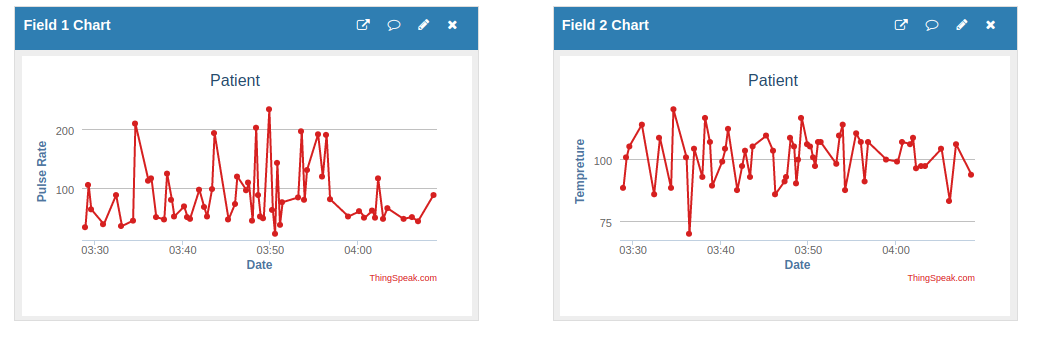
\includegraphics[scale=0.83]{chart.png}}
\caption{Gantt chart of the work execution process }
\label{fig18}
\end{figure}
